\documentclass[12pt, a4paper, simple]{eskdtext}

\usepackage{env}
\usepackage{hyperref}
\usepackage{_sty/gpi_lst}
\usepackage{_sty/gpi_toc}
\usepackage{_sty/gpi_p}
\usepackage{_sty/gpi_t}

% Код
\def \gpiDocTypeNum {81}
\def \gpiDocVer {00}
\def \gpiCode {\gpiLetterI\gpieLetterII\gpiLetterIII.\gpiStudentGroupName\gpiStudentGroupNum.\gpiStudentCard-0\gpiDocNum~\gpiDocTypeNum~\gpiDocVer}

\def \gpiDocTopic {\gpiFIObig\/F}

% Графа 1 (наименование изделия/документа)
\ESKDcolumnI {\ESKDfontIII \gpiTopic \\ \gpiDocTopic}

% Графа 2 (обозначение документа)
\ESKDsignature {\gpiCode}

% Графа 4 (литералы)
\ESKDcolumnIVfI {\gpiLetterI}
\ESKDcolumnIVfII {\gpieLetterII}
\ESKDcolumnIVfIII {\gpiLetterIII}

% Графа 9 (наименование или различительный индекс предприятия) задает команда
\ESKDcolumnIX {\gpiDepartment}

% Графа 11 (фамилии лиц, подписывающих документ) задают команды
\ESKDcolumnXIfI {\gpiStudentSurname}
\ESKDcolumnXIfII {\gpiTeacherSurname}
\ESKDcolumnXIfV {\gpiTeacherSurname}

\begin{document}
    \begin{ESKDtitlePage}
        \hspace{0pt}\\
        \vfill
        \begin{center}
            \textbf{\ESKDfontV \gpiTopic \\ \gpiDocTopic}
        \end{center}
        \vfill
        \hspace{0pt}\\
    \end{ESKDtitlePage}

    \tableofcontents                                
    \thispagestyle{empty} % удаляет нумерацию страниц, которую создает библиотека
    \newpage
    
    \section{Краткое функциональное описание системы}

Система обеспечивает первичный ввод типизированных документов бухгалтерского учета
(операция, сумма, базовая аналитика по операции) с последующей разноской (контировкой) данного документа в регистрационный журнал (РЖ). 

Далее из РЖ формируется книга счетов (КС), которая служит основанием для формирования балансовой отчетности (БО).
Данная система обеспечивает минимальный комплект~БО:
\begin{itemize}
    \item оборотно-сальдовая ведомость за период... по счету...;
    \item балансовая ведомость за период... по счету...;
    \item журнал-ордер за период... по счету... .
\end{itemize}

При формировании первичных документов используются картотеки справочного характера (справочники):
\begin{itemize}
    \item Определение первичных документов;
    \item Типовые хозяйственные операции (ТХО);
    \item План счетов (ПС);
    \item Виды аналитики;
    \item Коды аналитического учёта (КАУ).
\end{itemize}

\newpage

    \section{Материалы предварительного проектирования системы}
\subsection{Функциональная схема обработки данных}

\begin{figure}[!htb]
    \centering
    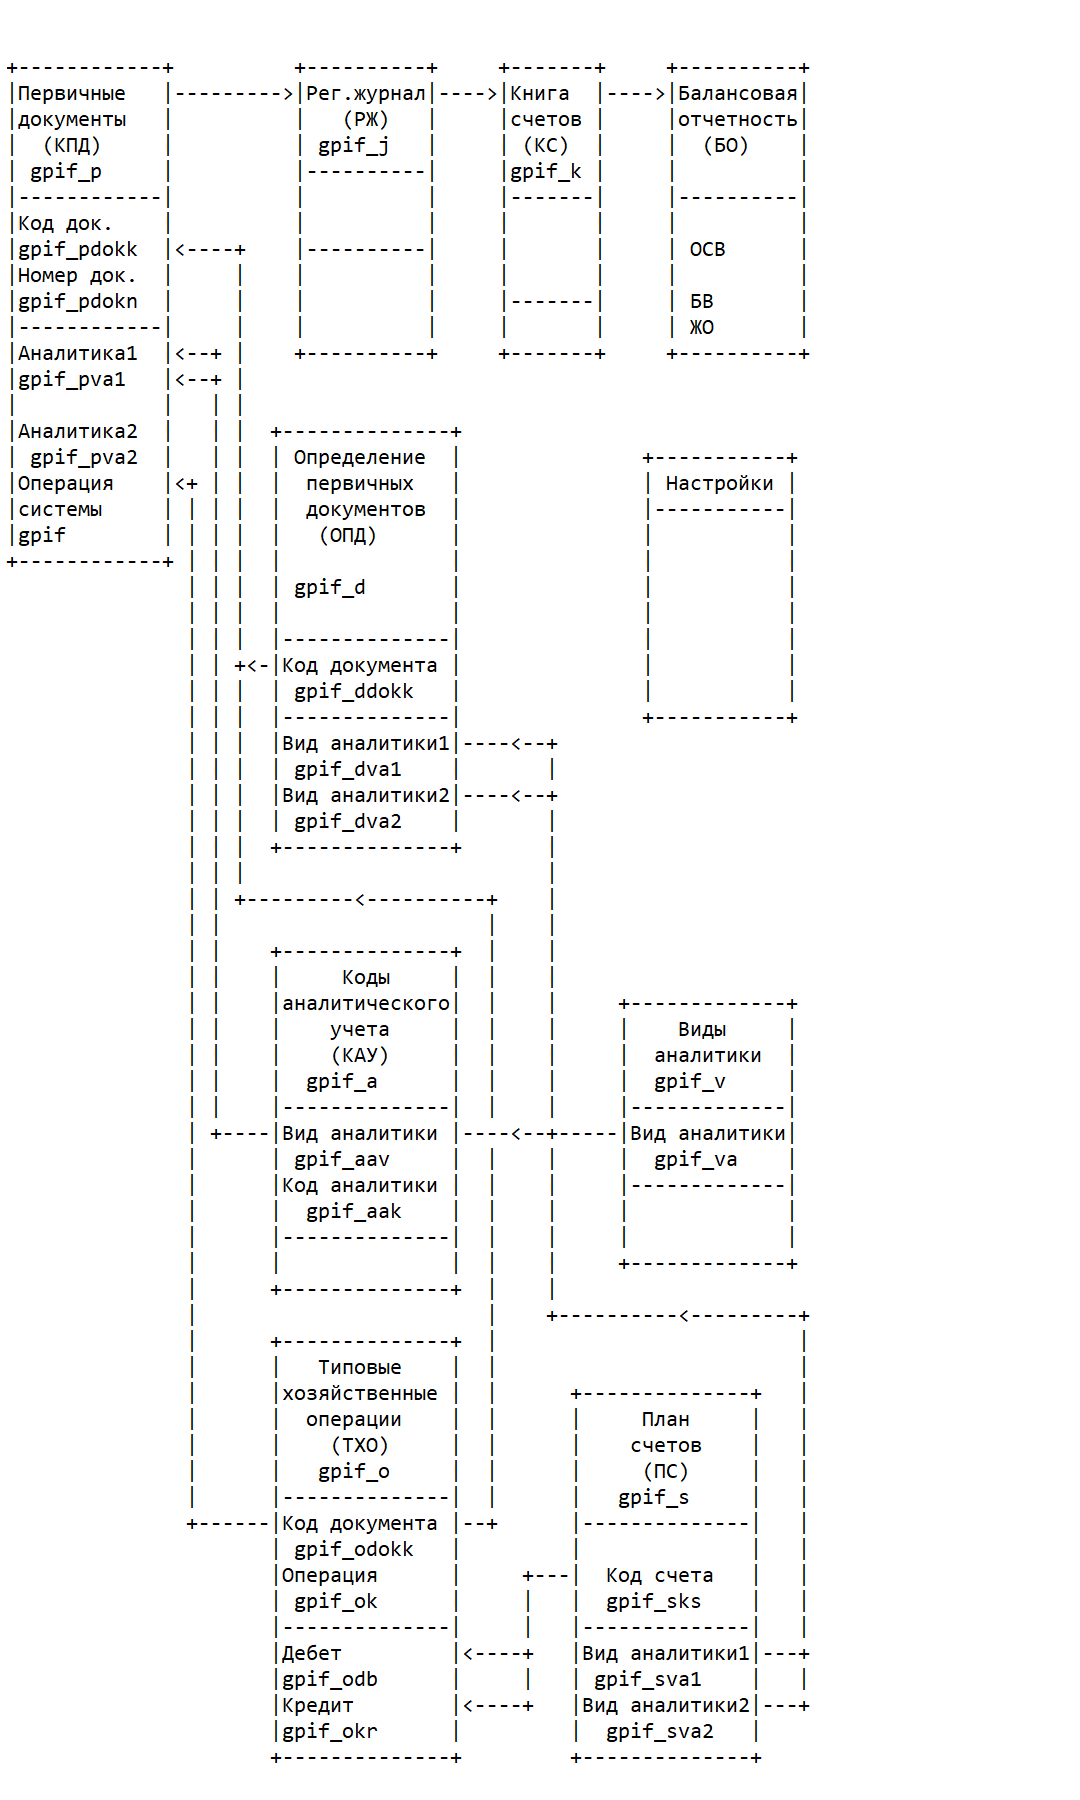
\includegraphics[height=19cm, width=14cm]
        {_assets/gpif_part2.png}
    \caption{Функциональная схема обработки данных}
\end{figure}

\subsection{Описание картотек}

Картотеки:

\begin{itemize}
    \item Первичные документы \gpiFIO\/f\_p;
    \item[]\hspace{0pt}
    \item Регистрационный журнал (РЖ) \gpiFIO\/f\_j;
    \item Книга счетов (КС) \gpiFIO\/f\_k;
    \item[]\hspace{0pt}
    \item Определение первичных документов \gpiFIO\/f\_d;
    \item Типовые хозяйственные операции (ТХО) \gpiFIO\/f\_o;
    \item План счетов (ПС) \gpiFIO\/f\_s;
    \item Коды аналитического учёта (КАУ) \gpiFIO\/f\_a;
    \item Виды аналитики \gpiFIO\/f\_v;
    \item[]\hspace{0pt}
    \item Настройки системы \gpiFIO\/f\_с. 
\end{itemize}

\begin{table}[h!p]
    \centering
    \scriptsize
    \caption{Первичные документы \gpiFIO\/f\_p}
    \begin{tabular}{|p{7cm}|p{7cm}|c|}

\hline
\multicolumn{1}{|c}{\textbf{Реквизит}}
&\multicolumn{1}{|c}{\textbf{Обозначение}}  
&\multicolumn{1}{|p{1.6cm}|}{\textbf{Тип и значность}} 
\\ \hline

поле связи =0                       &\gpiFIO\/f\_p0     &n1     \\ \hline
код документа < --- d               &\gpiFIO\/f\_pdokk  &c3     \\ \hline
номер документа                     &\gpiFIO\/f\_pdokn  &n5     \\ \hline
дата документа                      &\gpiFIO\/f\_pdokd  &d8     \\ \hline
вид аналитики 1 *d                  &\gpiFIO\/f\_pav1   &c3     \\ \hline
тип аналитики 1 =д, к, x            &\gpiFIO\/f\_pavt1  &c1     \\ \hline
аналитика код 1 < --- a             &\gpiFIO\/f\_pak1   &c10    \\ \hline
вид аналитики2                      &\gpiFIO\/f\_pav2   &c3     \\ \hline
тип аналитики2                      &\gpiFIO\/f\_pavt2  &c1     \\ \hline
аналитика код2                      &\gpiFIO\/f\_pak2   &c10    \\ \hline
вид аналитики3                      &\gpiFIO\/f\_pav3   &c3     \\ \hline
тип аналитики3                      &\gpiFIO\/f\_pavt3  &c1     \\ \hline
аналитика код3                      &\gpiFIO\/f\_pak3   &c10    \\ \hline
сумма                               &\gpiFIO\/f\_prub   &n10    \\ \hline
операции                            &\gpiFIO\/f\_pto    &c10    \\ \hline
дебет счет *o                       &\gpiFIO\/f\_pdb    &n2     \\ \hline
дебет счет субсчет наименование *o  &\gpiFIO\/f\_pdbn   &c10    \\ \hline
кредит *o                           &\gpiFIO\/f\_pkr    &n2     \\ \hline
кредит название *o                  &\gpiFIO\/f\_pkrn   &c10    \\ \hline

    \end{tabular}
\end{table}

\begin{table}[h!p]
    \centering
    \scriptsize
    \caption{Регистрационный журнал (РЖ) \gpiFIO\/f\_j}
    \begin{tabular}{|p{7cm}|p{7cm}|c|}

\hline
\multicolumn{1}{|c}{\textbf{Реквизит}}
&\multicolumn{1}{|c}{\textbf{Обозначение}}  
&\multicolumn{1}{|p{1.6cm}|}{\textbf{Тип и значность}} 
\\ \hline

поле связи	=0                      &\gpiFIO\/f\_j0     &n1     \\ \hline
дата операции                       &\gpiFIO\/f\_jdata  &d8     \\ \hline
код оправдательного документа       &\gpiFIO\/f\_jdokk  &c3     \\ \hline
номер документа                     &\gpiFIO\/f\_jdokn  &n10    \\ \hline
дата документа                      &\gpiFIO\/f\_jdokd  &d8     \\ \hline
содержание операции                 &\gpiFIO\/f\_jto    &c10    \\ \hline
дебет, счет                         &\gpiFIO\/f\_jdb    &n2     \\ \hline
дебет, название                     &\gpiFIO\/f\_jdbn   &c10    \\ \hline
кредит, счет                        &\gpiFIO\/f\_jkr    &n2     \\ \hline
кредит название                     &\gpiFIO\/f\_jkrn   &c10    \\ \hline
Сумма                               &\gpiFIO\/f\_jrub   &n10    \\ \hline

    \end{tabular}
\end{table}

\begin{table}[h!p]
    \centering
    \scriptsize
    \caption{Книга счетов(КС) \gpiFIO\/f\_k}
    \begin{tabular}{|p{7cm}|p{7cm}|c|} 

\hline
\multicolumn{1}{|c}{\textbf{Реквизит}}
&\multicolumn{1}{|c}{\textbf{Обозначение}}  
&\multicolumn{1}{|p{1.6cm}|}{\textbf{Тип и значность}} 
\\ \hline

поле связи  =0                      &\gpiFIO\/f\_k0     &n1     \\ \hline
дата операции                       &\gpiFIO\/f\_kdata  &d8     \\ \hline
код оправдательного документа       &\gpiFIO\/f\_kdokk  &c3     \\ \hline
номер документа                     &\gpiFIO\/f\_kdokn  &n10    \\ \hline
дата документа                      &\gpiFIO\/f\_kdokd  &d8     \\ \hline
операции                            &\gpiFIO\/f\_kto    &c10    \\ \hline
счет                                &\gpiFIO\/f\_ks     &n2     \\ \hline
счёт название                       &\gpiFIO\/f\_ksn    &c10    \\ \hline
кор. счёт                           &\gpiFIO\/f\_kks    &n2     \\ \hline
кор. счет наименование              &\gpiFIO\/f\_kksn   &c10    \\ \hline
сумма дб                            &\gpiFIO\/f\_kdb    &n10    \\ \hline
сумма кр                            &\gpiFIO\/f\_kkr    &n10    \\ \hline

    \end{tabular}
\end{table}

\begin{table}[h!p]
    \centering
    \scriptsize
    \caption{Определение первичных документов \gpiFIO\/f\_d}
    \begin{tabular}{|p{7cm}|p{7cm}|c|}

\hline
\multicolumn{1}{|c}{\textbf{Реквизит}}
&\multicolumn{1}{|c}{\textbf{Обозначение}}  
&\multicolumn{1}{|p{1.6cm}|}{\textbf{Тип и значность}} 
\\ \hline

поле связи =0                       &\gpiFIO\/f\_d0     &n1     \\ \hline
код документа                       &\gpiFIO\/f\_dk     &c3     \\ \hline
наименование документа              &\gpiFIO\/f\_dn     &c10    \\ \hline
вид аналитики 1 < --- v             &\gpiFIO\/f\_dav1   &c3     \\ \hline
тип аналитики 1 =д, к, x            &\gpiFIO\/f\_davt1  &c1     \\ \hline
виды аналитики 2                    &\gpiFIO\/f\_dav2   &c3     \\ \hline
тип аналитики 2                     &\gpiFIO\/f\_davt2  &c1     \\ \hline
вид аналитики 3                     &\gpiFIO\/f\_dav3   &c3     \\ \hline
тип аналитики 2                     &\gpiFIO\/f\_davt3  &c1     \\ \hline

    \end{tabular}
\end{table}

\begin{table}[h!p]
    \centering
    \scriptsize
    \caption{Типовые хозяйственные операции(ТХО) \gpiFIO\/f\_o}
    \begin{tabular}{|p{7cm}|p{7cm}|c|}

\hline
\multicolumn{1}{|c}{\textbf{Реквизит}}
&\multicolumn{1}{|c}{\textbf{Обозначение}}  
&\multicolumn{1}{|p{1.6cm}|}{\textbf{Тип и значность}} 
\\ \hline

поле связи =0                       &\gpiFIO\/f\_o0     &n1     \\ \hline
код документа < --- d               &\gpiFIO\/f\_odok   &c3     \\ \hline
Операции                            &\gpiFIO\/f\_ok     &c10    \\ \hline
дебет, счёт < --- s\_1              &\gpiFIO\/f\_odb    &n2     \\ \hline
дебет, название * s\_1              &\gpiFIO\/f\_odbn   &c10    \\ \hline
кредит < --- s\_2                   &\gpiFIO\/f\_okr    &n2     \\ \hline
кредит, название * s\_2             &\gpiFIO\/f\_okrn   &c10    \\ \hline

    \end{tabular}
\end{table}

\begin{table}[h!p]
    \centering
    \scriptsize
    \caption{План счетов(ПС) \gpiFIO\/f\_s}
    \begin{tabular}{|p{7cm}|p{7cm}|c|}

\hline
\multicolumn{1}{|c}{\textbf{Реквизит}}
&\multicolumn{1}{|c}{\textbf{Обозначение}}  
&\multicolumn{1}{|p{1.6cm}|}{\textbf{Тип и значность}} 
\\ \hline

поле связи =0                       &\gpiFIO\/f\_s0     &n1     \\ \hline
счет                                &\gpiFIO\/f\_sk     &n2     \\ \hline
название счета                      &\gpiFIO\/f\_sn     &c10    \\ \hline
тип счета = а, п, x                 &\gpiFIO\/f\_styp   &c1     \\ \hline
вид аналитики 1 из V                &\gpiFIO\/f\_sav1   &c3     \\ \hline
вид аналитики 2 из V                &\gpiFIO\/f\_sav2   &c3     \\ \hline

    \end{tabular}
\end{table}

\begin{table}[h!p]
    \centering
    \scriptsize
    \caption{Коды аналитического учёта(КАУ) gpia\_a}
    \begin{tabular}{|p{7cm}|p{7cm}|c|}

\hline
\multicolumn{1}{|c}{\textbf{Реквизит}}
&\multicolumn{1}{|c}{\textbf{Обозначение}}  
&\multicolumn{1}{|p{1.6cm}|}{\textbf{Тип и значность}} 
\\ \hline

поле связи =0                       &\gpiFIO\/f\_a0     &n1     \\ \hline
вид аналитики                       &\gpiFIO\/f\_av     &c3     \\ \hline
вид аналитики                       &\gpiFIO\/f\_ak     &c10    \\ \hline

    \end{tabular}
\end{table}

\begin{table}[h!p]
    \centering
    \scriptsize
    \caption{Виды аналитики \gpiFIO\/f\_v}
    \begin{tabular}{|p{7cm}|p{7cm}|c|}

\hline
\multicolumn{1}{|c}{\textbf{Реквизит}}
&\multicolumn{1}{|c}{\textbf{Обозначение}}  
&\multicolumn{1}{|p{1.6cm}|}{\textbf{Тип и значность}} 
\\ \hline

поле связи =0                       &\gpiFIO\/f\_v0     &n1     \\ \hline
вид аналитики                       &\gpiFIO\/f\_vk     &c3     \\ \hline
название вида аналитики             &\gpiFIO\/f\_vn     &c10    \\ \hline

    \end{tabular}
\end{table}

\begin{table}[h!p]
    \centering
    \scriptsize
    \caption{Настройки системы gpia\_c}
    \begin{tabular}{|p{7cm}|p{7cm}|c|}

\hline
\multicolumn{1}{|c}{\textbf{Реквизит}}
&\multicolumn{1}{|c}{\textbf{Обозначение}}  
&\multicolumn{1}{|p{1.6cm}|}{\textbf{Тип и значность}} 
\\ \hline

поле связи =0                       &\gpiFIO\/f\_c0     &n1     \\ \hline
дата текущая                        &\gpiFIO\/f\_cdatt  &d8     \\ \hline
интервал с                          &\gpiFIO\/f\_cdats  &d8     \\ \hline
интервал до                         &\gpiFIO\/f\_cdatd  &d8     \\ \hline
cчёт                                &\gpiFIO\/f\_cs     &n2     \\ \hline
название счёта                      &\gpiFIO\/f\_csn    &c10    \\ \hline
название фирмы                      &\gpiFIO\/f\_cfirm  &c10    \\ \hline

    \end{tabular}
\end{table}

\newpage

\subsection{Описание работ}

\begin{table}[h!p]
    \centering
    \scriptsize
    \caption{Описание работ}
    \begin{tabular}{|p{6cm}|p{11cm}|} 

% = = = = = = = = = =

\hline
\multicolumn{1}{|c}{\textbf{Группа работ}}
&\multicolumn{1}{|c|}{\textbf{Работы}}
\\ \hline

% = = = = = = = = = =

Формирование и разноска первичных \par
документов \par
\hspace{0pt} \par
\textbf{\gpiFIO\/f\_документы}
&
- \gpiFIO\/f\_ввод текущей даты \par
- \gpiFIO\/f\_ввод и разноска первичных документов
\\ \hline

% = = = = = = = = = =

Работа с регистрационным журналом \par
\hspace{0pt} \par
\textbf{\gpiFIO\/f\_РЖ}
&
- \gpiFIO\/f\_просмотр РЖ \par
- \gpiFIO\/f\_формирование КС и РЖ \par
- \gpiFIO\/f\_просмотр КС \par
- \gpiFIO\/f\_сформировать КС на печать \par
- \gpiFIO\/f\_просмотр КС для печати
\\ \hline

% = = = = = = = = = =

Формирование балансовой отчетности \par
\hspace{0pt} \par
\textbf{\gpiFIO\/f\_БО}
&
- \gpiFIO\/f\_опеделение отчетных форм \par
- \gpiFIO\/f\_сформировать КС на печать \par
- \gpiFIO\/f\_просмотр КС для печати \par
- \gpiFIO\/f\_сформировать ОСВ \par
- \gpiFIO\/f\_просмотр ОСВ \par
- \gpiFIO\/f\_сформировать Ж-О \par
- \gpiFIO\/f\_просмотр Ж-О \par
- \gpiFIO\/f\_сформировать БВ \par
- \gpiFIO\/f\_просмотр БВ
\\ \hline

% = = = = = = = = = =

Сопровождение картотек-справочников \par
\hspace{0pt} \par
\textbf{\gpiFIO\/f\_картотеки}
&
- \gpiFIO\/f\_определение первичных документов \par
- \gpiFIO\/f\_типовые хозяйственные операции (ТХО) \par  
- \gpiFIO\/f\_план счетов (ПС) \par
- \gpiFIO\/f\_виды аналитики \par 
- \gpiFIO\/f\_коды аналитического учёта (КАУ) \par
- \gpiFIO\/f\_настройка АРМа
\\ \hline

% = = = = = = = = = =

Ведение архивов \par
\hspace{0pt} \par
\textbf{\gpiFIO\/f\_архив}
&
- \gpiFIO\/f\_копия АРМ \par
- \gpiFIO\/f\_восстановление АРМ 
\\ \hline

% = = = = = = = = = =

    \end{tabular}
\end{table}

\newpage

    \section{Эксплуатационное описание системы}

\subsection{Функциональная схема обработки данных с использованием инструментальной среды}
\subsection{Описание картотек с использованием инструментальной среды}
\subsection{Скриншоты меню}
\subsection{Скриншоты картотек}
\subsection{Образцы первичных документов}
\subsection{Образцы печатных форм}

% \newpage

    \section{Электронная версия разработанной системы}

\newpage

\end{document}
